\usetikzlibrary{arrows}
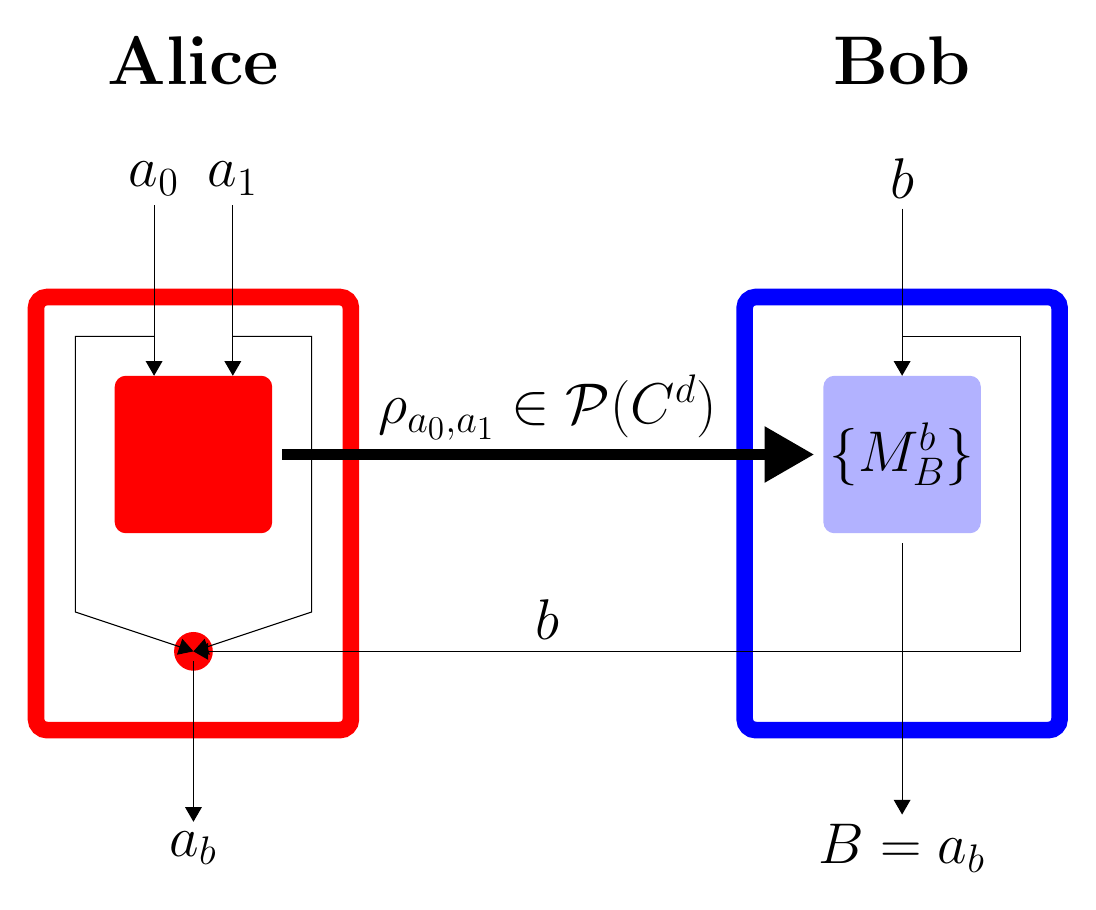
\begin{tikzpicture}

\fill[rounded corners,color=red]  (-4,2.5) rectangle (-2,0.5);
\fill[rounded corners,color=blue,opacity=0.3]  (5,2.5) rectangle (7,0.5);

\node at (-2.5,2) {};
\coordinate (v6) at (6,2.5) {};
\node (v7) at (6,0.5) {};
\node (v1) at (-3.5,5) {\huge $a_0$};
\node (v3) at (-2.5,5) {\huge $a_1$};
\node (v5) at (6,5) {\huge$b$};
\node (v8) at (6,-3.5) {\huge $B=a_b$};
\node (v19) at (-2,1.5) {};
\draw[rounded corners,color=red,line width=6pt]  (-5,3.5) rectangle (-1,-2);
\draw[rounded corners,color=blue,line width=6pt]  (4,3.5) rectangle (8,-2);
\coordinate (v2) at (-3.5,2.5) {};
\coordinate (v4) at (-2.5,2.5) {};
\draw [-triangle 60] (v1) edge (v2);
\draw [ -triangle 60] (v3) edge (v4);
\draw [ -triangle 60] (v5) edge (v6);
\draw [ -triangle 60] (v7) edge (v8);
\coordinate (v9) at (-3.5,3) {};
\coordinate (v10) at (-4.5,3) {};
\coordinate (v11) at (-4.5,-0.5) {} {};
\coordinate (v16) at (-1.5,3) {};
\coordinate (v15) at (-2.5,3) {};
\coordinate (v17) at (-1.5,-0.5) {} {};
\coordinate (v12) at (-3,-1) {} {} {} {};
\node (v13) at (-3,-1) {};
\node (v14) at (-3,-3.5) {\huge $a_b$};
\coordinate (v18) at (7.5,-1) {};
\fill[ color=red ] (v12) circle (7pt);
\draw [-triangle 60] (v13) edge  (v14);
\node (v20) at (5,1.5) {};
\draw [-triangle 60,line width=4pt] (v19) edge node[above]{\huge $\rho_{a_0,a_1}\in \mathcal{P}(\mathbb{C}^d)$} (v20);
\node at (-3,6.5) {\Huge \bf Alice};
\node at (6,6.5) {\Huge \bf Bob};
\coordinate (v21) at (6,3) {};
\coordinate (v22) at (7.5,3) {};
\draw [-triangle 60] (v21) -- (v22) -- (v18) -- (v12);
\node at (1.5,-0.6) {\huge $b$};
\node at (6,1.5) {\huge $\{M_B^b\}$};
\draw [-triangle 60] (v15) -- (v16) -- (v17) -- (v12);
\draw [-triangle 60] (v9) -- (v10) -- (v11) -- (v12);
\end{tikzpicture}